\section{System}
\label{sec:sys}

Our \ql system implementation builds on Apache Spark with GraphX.  We
selected Spark because it is a popular open-source system, and because
of its in-memory processing approach.  All \tg operations are
available through the public API of the \ql library, and may be used
like any other library in an Apache Spark application.  \insql{TGraph}
is the main abstract class that all physical representations extend.
An excerpt of the API, where VD is the vertex attribute and ED is the
edge attribute type:

\begin{lstlisting}
def slice(bound: Interval): TGraph[VD, ED]
def aggregate(window: WindowSpecification, vquant: Quantification, equant: Quantification, vAggFunc: (VD, VD) => VD, eAggFunc: (ED, ED) => ED)(vgroupby: (VertexId, VD) => VertexId): TGraph[VD, ED]
def union(other: TGraph[VD, ED]): TGraph[Set[VD], Set[ED]]
\end{lstlisting}

\subsection{Physical Represenatations}
\label{sec:sys:datastructs}

We considered four in-memory \tg representations that differ in
compactness, but also, perhaps more importantly, in the kind of
locality they prioritize. With {\em structural locality}, neighboring
vertices (resp. edges) of the same representative graph are laid out
together, while with {\em temporal locality}, consecutive states of
the same vertex (resp. edge) are laid out
together~\cite{DBLP:journals/tos/MiaoHLWYZPCC15}.  VertexEdgeGraph
(VE) is a direct translation of the vertex-edge relations model and
the most compact representation.  While VE is a logical represenation
and does not necessitate a particular order of tuples on disk, we opt
for a physical layout in which all tuples corresponding to the same
vertex (resp. edge) are laid out consecutively, and so VE preserves
temporal localilty.  SnapshotGraph (SG), a representation in which
each representative graph is stored explicitly, naturally preserves
structural locality, but temporal locality is lost. OneGraph (OG)
stores all vertices and edges of an evolving graph once, in a single
data structure.  This representation emphasizes temporal locality,
while also preserving structural locality.  HybridGraph (HG) trades
compactness for better structural locality, by aggregating together
several consecutive RGs, and computing a OneGraph for each graph
cluster.  We can convert from one representation to any other at small
or no cost, so it is useful to think of them as access methods in the
context of individual operations.

\begin{table*}[t]
\centering
\small
\begin{tabular}{ p{1.6cm} | p{3.5cm} | p{3.5cm} | p{3.5cm} | p{3.5cm} }
\hline
\multicolumn{1}{l|}{\bfseries Operation} & \multicolumn{1}{c|}{\bfseries VE} & \multicolumn{1}{c|}{\bfseries SG} & \multicolumn{1}{c|}{\bfseries OG} & \multicolumn{1}{c|}{\bfseries HG} \\ \hline
slice & filter V and E; modify periods to be within slice interval & slice sequence of RGs & filter indices in bitsets & slice sequence of OGs and filter indices in remaining OGs \\ \hline
select & filter V ad E; enforce FK constraint & only when predicate not on interval: filter V and E of each RG & N/A & N/A \\ \hline
project & apply projection to each element of defined projection; coalesce & apply projection to each element within each RG; coalesce and recompute & N/A & N/A \\ \hline
aggregate (non-structural) & split each vertex/edge by window; reduce by window key; filter those under quantification threshold; enforce FK constraint & map each RG to windows; group vertices/edges in each window into one RG, filtering by quantification & only structure: for each vertex/edge map indices in bitsets to corresponding windows; filter by quantification threshold; enforce FK constraint & only structure: combine OGs as necessary to group into windows; map indices in bitsets; filter by quantification threshold; enforce FK constraint \\ \hline
aggregate (with structural) & map each vertex to new id; join edges with new vertices to get new id; rest as above & within each window map vertices and edge triplets to new ids; rest as above & N/A & N/A \\ \hline
union & compute combined intervals; split each vertex/edge by new intervals; full outer join & compute combined intervals; combine RGs in corresponding intervals; full outer join & structure only: remap bitsets to new intervals; union vertices/edges from two graphs and reduce by key to combine bitsets & structure only: combine OGs as necessary; rest as in OG \\ \hline
intersection & compute intervals; split each vertex/edge by new interval; inner join & compute intervals; inner join of vertices/edges from corresponding intervals & structure only: like union but with bitset intersection & structure only: like union but with bitset intersection \\ \hline
analytics (pagerank, shortest paths, etc.) & N/A & compute for each RG & compute for all periods simultaneously & compute for all periods within each OG simultaneously \\ 
\hline
\end{tabular}
\caption{Operations.}
\label{tab:operations}
\end{table*}

{\bf VertexEdgeGraph (VE).} VEGraph is a direct translation of the
vertex-edge TGraph data model: one RDD contains all the vertices and
another all the edges.  The attributes are treated as single nested
attributes for vertices and edges each, consistent with the GraphX
API.  The main advantage of this schema-less attribute representation
is that it can easily deal with schema evolution and leaves the
details of attribute processing to the user.  The VE representation
supports all the algebraic operations on TGraph (see
Table~\ref{tab:operations}) but cannot support analytics.  As we will
show, due to compactness this physical representation is the most
efficient for many operations.

{\bf SnapshotGraph (SG).} The simplest way to represent an evolving
graph is by representing each representative graph individually, a
direct translation of our RG logical data model.  We call this data
structure SnapshotGraph (for historical reasons), or SG for short. An
example of an SG is depicted in Figure~\ref{fig:tg_rg}.  SG is a
collection of GraphX graphs, where vertices and edges store the
attribute values for the specific time interval.  This representation
supports all the operations defined for TGraphs, with the exception of
\insql{select}. \insql{select} is only supported in cases without a
predicate on the time period.  To construct SG from V and E we
iteratively select from V and E for each RG period.

While the SG representation is simple, it is not compact, considering
that in many real-world evolving graphs there is a 80\% or larger
similarity between consecutive
snapshots~\cite{DBLP:journals/tos/MiaoHLWYZPCC15}.  In a distributed
architecture, however, this data structure provides some benefits as
operations on it can be easily parallelized, by assigning different
RGs to different workers, or by partitioning an RG across workers.
Without \ql a user wishing to analyze evolving graphs could use the SG
approach at the cost of poor performance on most operations.

\begin{figure}[t!]
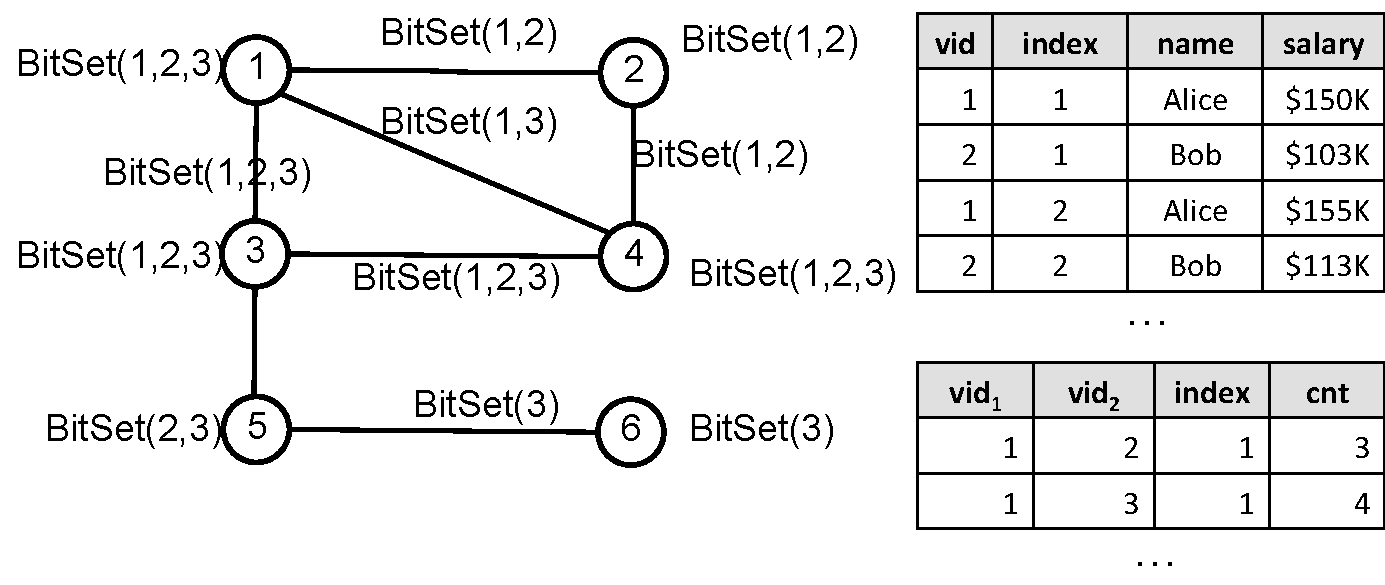
\includegraphics[width=3in]{figs/ogc.pdf}
\caption{OG representation of T1 from~\ref{fig:tg_ve}.}
\label{fig:ogc}
\end{figure}

{\bf OneGraph (OG).}  The most topologically compact representation is
to store each vertex {\em and} each edge only once for the whole
evolving graph, by taking a union of the vertex and edge sets.  The
OneGraph data structure, or OG for short, depicted in
Figure~\ref{fig:ogc}, uses this representation in our system.  The
drawback is that OG is much denser than individual graphs of SG.  OG
represents only the graph structure, which is sufficient for many
graph analytics.  As a result, this data structure supports
operations only on topology: analytics and aggregation/union/intersection
for graphs with no attributes or when attributes are not relevant for
analysis.  To construct OG vertices and edges from V and E relations
each are grouped by key and mapped to bitsets to represent
presence/absence in each time period of \tg in a single GraphX graph.
In general, because OG represents topology only, many fewer periods
need be represented and computed than there are RGs in \tg.  The
reduction depends on the rate and nature of the graph evolution.  For
completeness, OG supports all other operations through inheritance
from abstract parent, which are carried out on V and E relations.

{\bf HybridGraph (HG).} As an intermediate representation between SG
and OG, we implement the HybridGraph (HG) data structure.  HG is a
series of OGs, with each OG representing some number of temporally
adjacent RGs.  In our current implementation each OG in the sequence
corresponds to the same number of temporally adjacent graphs.  This is
the simplest clustering method, yet, as we will see in
Section~\ref{sec:exp}, it already improves performance compared to OG.
However, we also observed that placing the same number of graphs into
each cluster often results in unbalanced cluster sizes.  This is
because networks commonly exhibit strong temporal skew, with later RGs
being significantly larger than earlier ones.  Consequently, we are
currently working on more sophisticated clustering approaches that
would lead to better balance, and ultimately to better performance.
Like OG, this representation only supports topology-based analyses,
need not represent every RG but only structure-based changes, and
supports all other operations through inheritance.

\subsection{Maintenance Operations}
\label{sec:sys:maint}

\begin{table}
\small
\begin{tabular}{ l | p{4cm} | c }
\hline
\multicolumn{1}{l|}{\bfseries Operation} & \multicolumn{1}{c|}{\bfseries Requires Coalesced Input} & \multicolumn{1}{c}{\bfseries Uncoalesces} \\ \hline
slice & no & no \\ \hline
select & only if predicate incl. interval & no \\ \hline
project & no & yes \\ \hline
aggregate & only if structural group by is used and includes interval & yes \\ \hline
union & no & yes \\ \hline
intersection & no & yes \\ \hline
analytics & no & yes \\
\hline
\end{tabular}
\caption{Coalesce analysis.}
\label{tab:coalesce}
\end{table}

{\bf Coalescing.}  The TGraph logical data model is temporally
coalesced.  Portal supports both eager and lazy coalescing, with lazy
being the default behavior.  The final output is always coalesced.
For most operations, correctness of the operation does not depend on
whether the data is or is not coalesced in advance.  For example,
\insql{slice} operation is agnostic to whether a TGraph is coalesced
and does not change the coalesce state.  \insql{select} operation, on
the other hand, is only correct if the data is coalesced when the
selection predicate references the time period.  We analyzed all
operations for their coalescing requirements and whether the operation
causes uncoalescing (Table~\ref{tab:coalesce}).  Additionally, when
the operations are performed on multiple graphs (such as in SG and
HG), the result must also be coalesced to be correct, regardless of
the operation.

There are several different implementations possible for
implementation of the coalesce operation
(see~\cite{DBLP:conf/vldb/BohlenSS96} for detailed analysis in the
non-graph domain).  We use a partitioning method, where the relation
(V or E) is grouped by key, and within each group the tuples are
sorted and folded to produce the longest valid periods.  This approach
involves shuffling between partitions, one of the most computationally
expensive aspects of distributed systems, and thus lazy coalescing is
preferred in the general case.  As with duplicate elimintation, if the
coalesced output is expected to be significantly reduced in size, such
as after a project operation on a high volatility attribute,
performing coalesce eagerly before a time-consuming operation,
especially analytics, can be advantageous.

{\bf Foreign key constraint.}  The vertex-edge data model includes a
foreign key constraint from edges to vertices.  This constraint is
naturally maintained by most operations while performing operations on
V and E independently.  For \insql{select} and \insql{aggregate}
additional steps are required to insure correctness.  We modify E
tuples to enforce the foreign key constraint by joining on V, using
either a broadcast or hash join depending on the size of V.  Each edge
period is then modified to be the overlap of the periods of source and
destination vertices and the original edge period.  Because this step
is computationally expensive, it is only taken when necessary: when
\insql{select} has a predicate on V and when \insql{aggregate} has a
higher level of quantification for V than for E.  GraphX graphs
maintain foreign key constraint during subgraph operation and we make
use of this for all representations besides VE.

{\bf Partitioning.}  Graph partitioning can have a tremendous impact
on system performance.  A good partitioning strategy needs to (1) be
balanced, assigning an approximately equal number of units to each
partition, and (2) limit the number of cuts across partitions, to
reduce cross-partition communication.  In our experiments we compare
performance of SG, OG and HG with (1) no repartitioning after load,
and (2) with repartitioning using the 2D edge partitioning strategy
(E2D).  This strategy is available in GraphX and was used without
modification.  In E2D, a sparse edge adjacency matrix is partitioned
in two dimensions, guaranteeing a $2 \sqrt{n}$ bound on vertex
replication, where $n$ is the number of partitions. As has been shown
previously~\cite{DBLP:conf/osdi/GonzalezXDCFS14,MoffittTempWeb16}, E2D
provides good performance for Pregel-style analytics.

